% Auto-generated by 04_additional_analysis.R — do not edit
% y > 0: Underreacts  |  y < 0: Overreacts
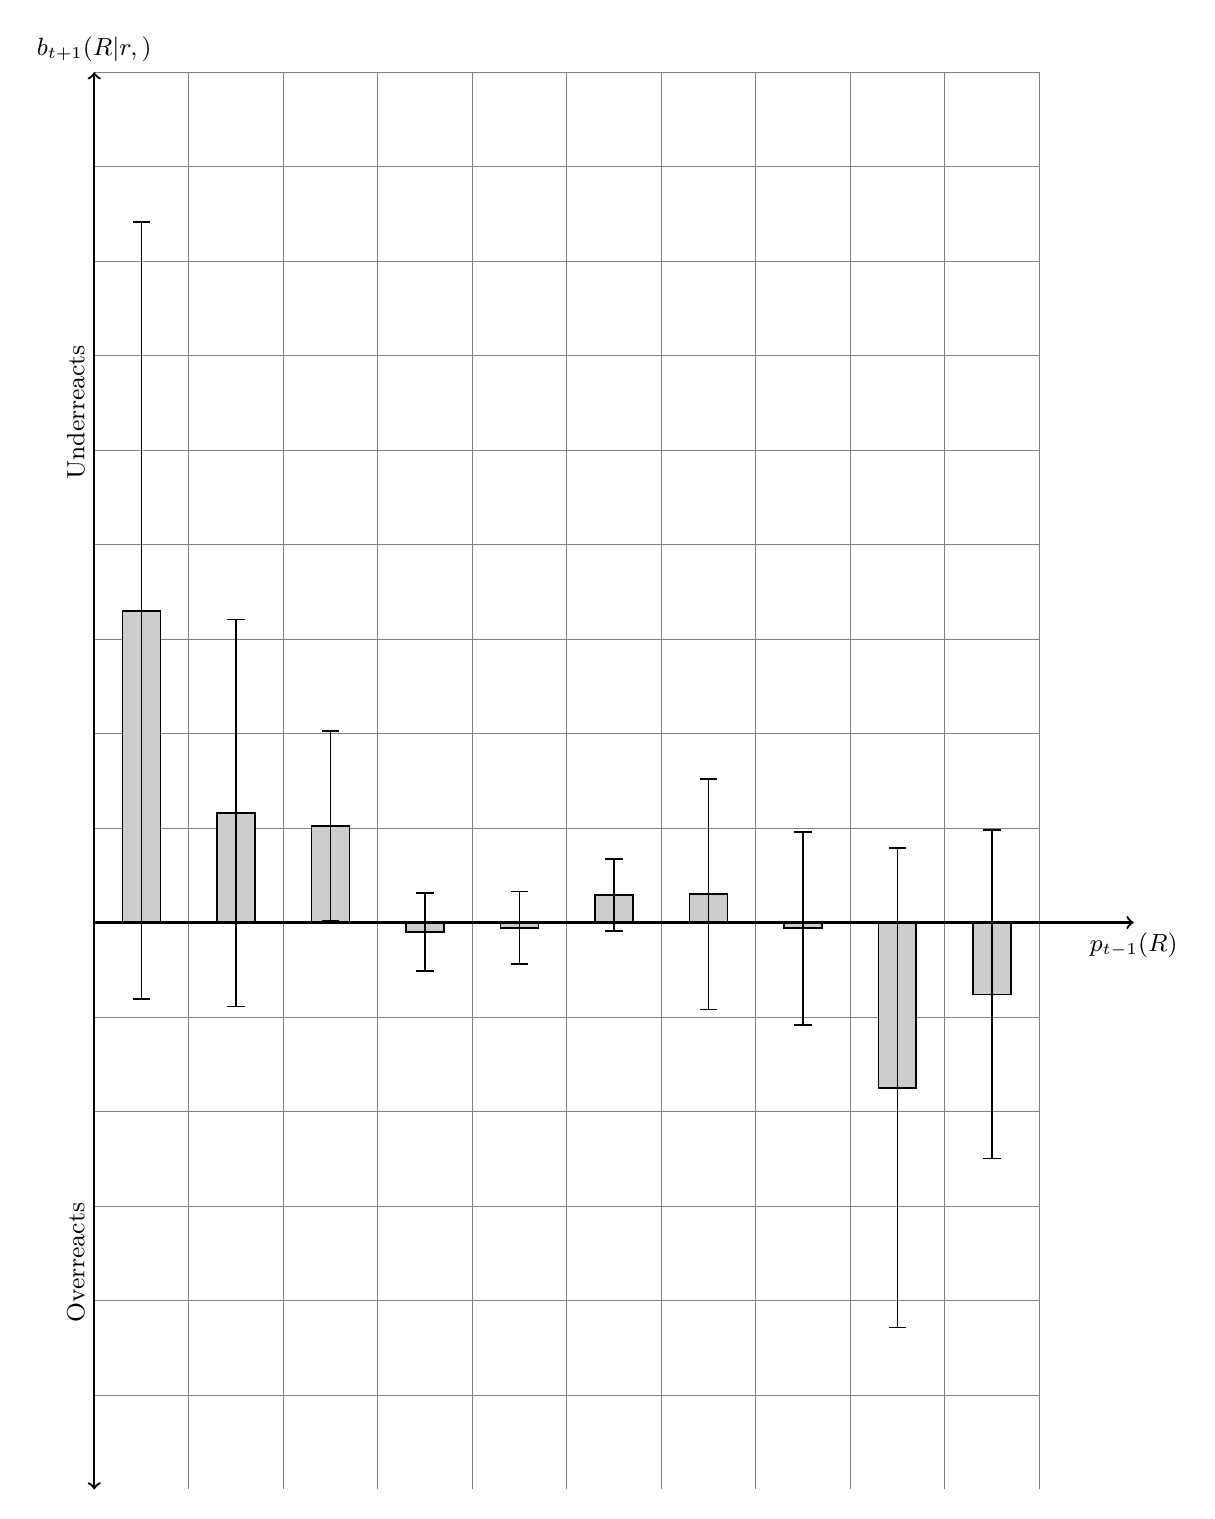
\begin{tikzpicture}[scale=12]
\draw[help lines,step=0.1] (0,-0.6) grid (1,0.9);
\filldraw[opaque,white!80!black] (0.03,0) rectangle (0.07,0.3300);
\draw[line width=0.6] (0.03,0) rectangle (0.07,0.3300);
\draw[line width=0.6,|-|] (0.05,-0.0821) -- (0.05,0.7421);
\filldraw[opaque,white!80!black] (0.13,0) rectangle (0.17,0.1160);
\draw[line width=0.6] (0.13,0) rectangle (0.17,0.1160);
\draw[line width=0.6,|-|] (0.15,-0.0896) -- (0.15,0.3216);
\filldraw[opaque,white!80!black] (0.23,0) rectangle (0.27,0.1025);
\draw[line width=0.6] (0.23,0) rectangle (0.27,0.1025);
\draw[line width=0.6,|-|] (0.25,0.0014) -- (0.25,0.2036);
\filldraw[opaque,white!80!black] (0.33,0) rectangle (0.37,-0.0100);
\draw[line width=0.6] (0.33,0) rectangle (0.37,-0.0100);
\draw[line width=0.6,|-|] (0.35,-0.0519) -- (0.35,0.0319);
\filldraw[opaque,white!80!black] (0.43,0) rectangle (0.47,-0.0056);
\draw[line width=0.6] (0.43,0) rectangle (0.47,-0.0056);
\draw[line width=0.6,|-|] (0.45,-0.0449) -- (0.45,0.0336);
\filldraw[opaque,white!80!black] (0.53,0) rectangle (0.57,0.0291);
\draw[line width=0.6] (0.53,0) rectangle (0.57,0.0291);
\draw[line width=0.6,|-|] (0.55,-0.0102) -- (0.55,0.0684);
\filldraw[opaque,white!80!black] (0.63,0) rectangle (0.67,0.0300);
\draw[line width=0.6] (0.63,0) rectangle (0.67,0.0300);
\draw[line width=0.6,|-|] (0.65,-0.0928) -- (0.65,0.1528);
\filldraw[opaque,white!80!black] (0.73,0) rectangle (0.77,-0.0060);
\draw[line width=0.6] (0.73,0) rectangle (0.77,-0.0060);
\draw[line width=0.6,|-|] (0.75,-0.1090) -- (0.75,0.0970);
\filldraw[opaque,white!80!black] (0.83,0) rectangle (0.87,-0.1750);
\draw[line width=0.6] (0.83,0) rectangle (0.87,-0.1750);
\draw[line width=0.6,|-|] (0.85,-0.4296) -- (0.85,0.0796);
\filldraw[opaque,white!80!black] (0.93,0) rectangle (0.97,-0.0760);
\draw[line width=0.6] (0.93,0) rectangle (0.97,-0.0760);
\draw[line width=0.6,|-|] (0.95,-0.2505) -- (0.95,0.0985);
\draw[line width=0.8,->]  (0,0) -- (1.1,0) node[below] {\small{$p_{t-1}(R)$}};
\draw[line width=0.8,<->] (0,-0.6) -- (0,0.9) node[above] {\small{$b_{t+1}(R|r,\xmark)$}};
\draw (0,0.54) node[above,rotate=90] {\small{Underreacts}};
\draw (0,-0.36) node[above,rotate=90] {\small{Overreacts}};
% ADD THEORY CURVE BELOW
\end{tikzpicture}
